\documentclass{article}
\usepackage[utf8]{inputenc}
\usepackage{graphicx}
\usepackage{amsmath}
\usepackage{amssymb}
\usepackage{amsthm}
\usepackage{bm}

\title{Computational Physics (physics760)\\Exercise 4}
\author{Ajay S. Sakthivasan, Dongjin Suh}
\date{November 25, 2022}

\begin{document}

\maketitle

\section{Applying HMC to multi-parameter fitting}

\begin{enumerate}
\item \textbf{Equations of Motion}\\
We have, 
\begin{equation}
    \mathcal{H}[p, \bm{\phi}] = \frac{p_0^2}{2} + \frac{p_1^2}{2} + \frac{p_2^2}{2} + \beta\chi^2(\bm{\phi}).
\end{equation}
Using Hamilton's equations,
\begin{align*}
    \rightarrow \dot{\phi_i} &= \frac{\partial}{\partial p_i}\mathcal{H}\\
    &= \frac{\partial}{\partial p_i} \left(\sum_{j=0}^2\frac{p_j^2}{2} + \beta\chi^2(\bm{\phi})\right)\\
    &= \sum_{j=0}^2 \delta_{ij} p_j = p_i
\end{align*}
\begin{equation}
\begin{split}
    \therefore \boxed{\dot{\phi_0} = p_0}\\
    \boxed{\dot{\phi_1} = p_1}\\
    \boxed{\dot{\phi_2} = p_2}
\end{split}
\end{equation}

\begin{align*}
    \rightarrow \dot{p_i} &= -\frac{\partial}{\partial\phi_i}\mathcal{H}\\
    &= -\frac{\partial}{\partial\phi_i} \left(\sum_{j=1}^3\frac{p_j^2}{2} + \beta\chi^2(\bm{\phi})\right)\\
    &= -\beta\frac{\partial}{\partial\phi_i} \left(\frac{1}{2} \sum_{k=1}^5 \frac{(f_k - f(m_{\pi,k},\bm{\phi}))^2}{\delta f_k^2}\right)\\
    &= \beta\sum_{k=1}^5\left(\frac{f_k - f(m_{\pi,k},\bm{\phi})}{\delta f_k^2} \frac{\partial}{\partial\phi_i}f(m_{\pi,k}, \bm{\phi})\right)\\
    \text{Using, } f(m_\pi, \bm{\phi}) &= \phi_0 + \phi_1 m_{\pi} + \phi_2 m_{\pi}^2\\
    \dot{p_i} &= \beta\sum_{k=1}^5\left(\frac{f_k - f(m_{\pi,k},\bm{\phi})}{\delta f_k^2}\sum_{j=0}^2\delta_{i,j}m_{\pi,k}^j\right)\\
    &= \beta\sum_{k=1}^5\left(\frac{f_k - f(m_{\pi,k},\bm{\phi})}{\delta f_k^2}m_{\pi,k}^i\right)\\
\end{align*}
\begin{equation}
\begin{split}
    \therefore &\boxed{\dot{p_0} = \beta\sum_{k=1}^5\frac{f_k - f(m_{\pi,k}, \bm{\phi})}{\delta f_k^2}}\\
    &\boxed{\dot{p_1} = \beta\sum_{k=1}^5\frac{f_k - f(m_{\pi,k}, \bm{\phi})}{\delta f_k^2}m_{\pi,k}}\\
    &\boxed{\dot{p_2} = \beta\sum_{k=1}^5\frac{f_k - f(m_{\pi,k}, \bm{\phi})}{\delta f_k^2}m_{\pi,k}^2}\\
\end{split}
\end{equation}

\item \textbf{Leapfrog Integrator}\\
The leapfrog integration was modified to accommodate the new system and figure \ref{fig:leapfrog} was obtained. We can see that the plot shows the expected quadratic behaviour for large molecular dynamics steps. But, this is not true for smaller molecular dynamics steps. This is fine since the quadratic relation is an asymptotic behaviour.\\

\begin{figure}[h!]
    \centering
    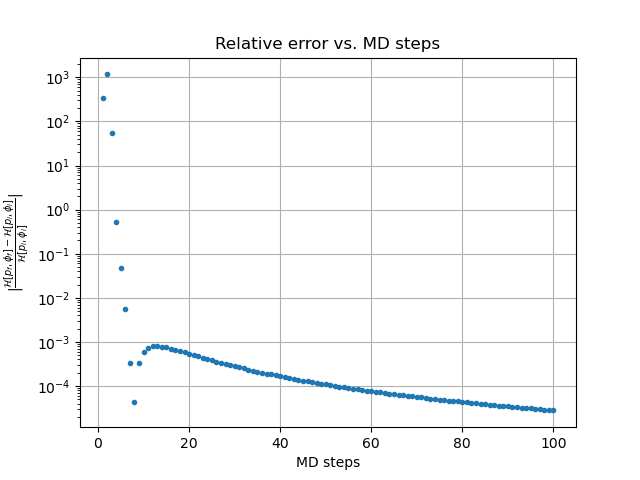
\includegraphics[width = .7\linewidth]{leapfrog.png}
    \caption{Relative error in the energy vs. MD steps}
    \label{fig:leapfrog}
\end{figure}

\item \textbf{HMC Algorithm}\\
Following this, we modified the code from previous week's submission to accommodate the new system for our HMC algorithm. This was then used to determine the values of $\phi$. With our code, we were able to achieve an acceptance of about $0.99$. Figure \ref{fig:hmctraj} shows the values of $\phi$ plotted against the HMC trajectory. Figure \ref{fig:mass} shows the values of the fit function plotted as a function of pion mass. We see that this plot is in good agreement with the given data. The best fit values and the corresponding errors are included in the code. The ``physical'' neutron mass is given by the fit function at $m_{\pi} = 0.134977 \text{MeV}$ as $912 \text{MeV}$. In the chiral limit, the fit function reduces to $\phi_0$ whose value is $757 \text{MeV}$. This is not particularly surprising to us, since in the chiral limit we expect the nucleon mass to reduce to the characteristic scale of \textit{QCD}, which is about $\sim 1 \text{GeV}$. However, the pion mass reducing to zero should be surprising with this explanation. Again, we should notice that the pion is a quasi-Goldstone boson and the Goldstone's theorem ensures that this boson is massless.

\begin{figure}[h!]
    \centering
    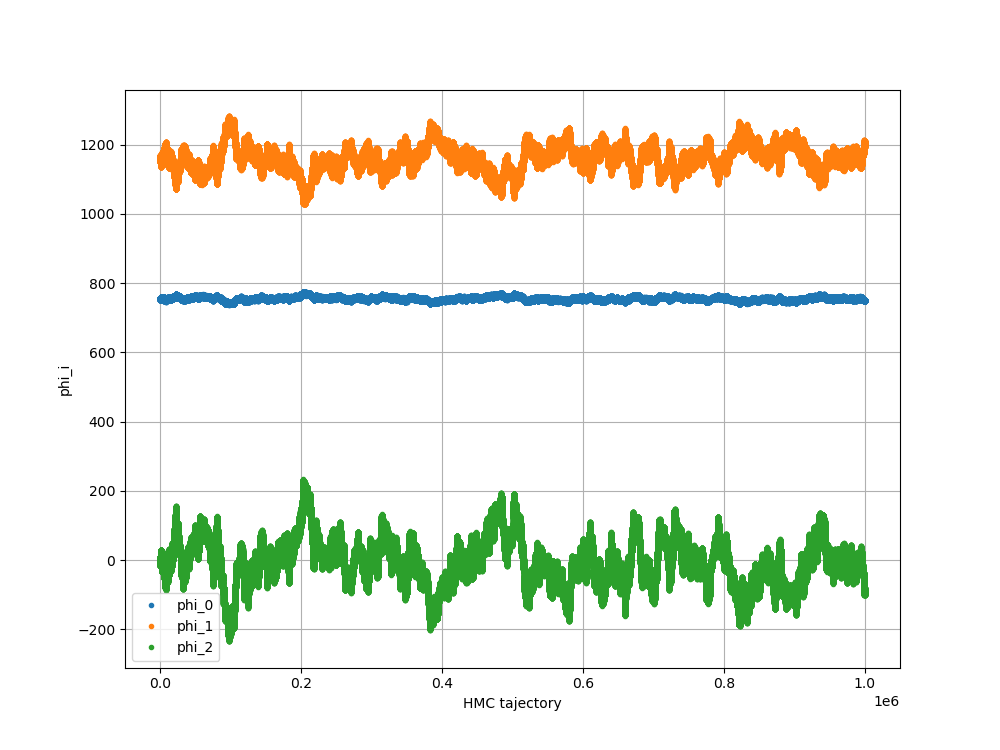
\includegraphics[width = .7\linewidth]{hmctraj.png}
    \caption{$\phi$ vs. HMC trajectory}
    \label{fig:hmctraj}
\end{figure}

\begin{figure}[h!]
    \centering
    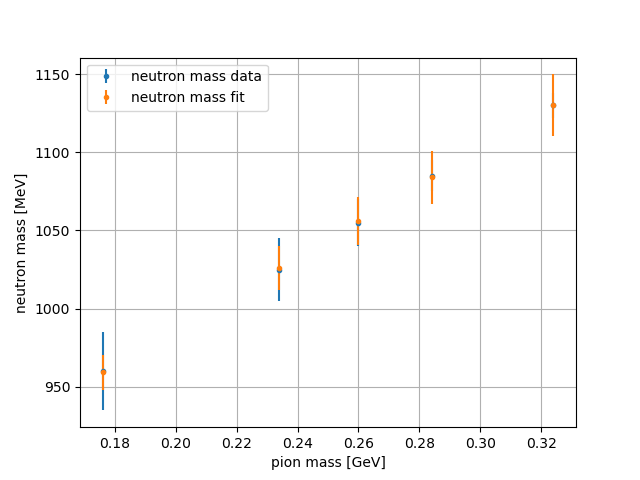
\includegraphics[width = .7\linewidth]{mass.png}
    \caption{Fit function vs. $\pi$ Mass}
    \label{fig:mass}
\end{figure}

\end{enumerate}

\end{document}